\begin{mychapter}{Deployment in AWS}

\begin{mysection}{Deployment tramite Infrastructure-as-Code (Terraform)}
Al fine di automatizzare e rendere riproducibile l'infrastruttura Cloud, è stato creato uno script Terraform per effettuare il provisioning delle risorse su Amazon Web Services (AWS).
Questa metodologia, nota come \textit{Infrastructure-as-Code} (IaC), garantisce che la configurazione del cloud sia scritta in file dichiarativi, riducendo l'errore umano.

I file Terraform implementati (\texttt{main.tf}, \texttt{variables.tf}, \texttt{outputs.tf}) descrivono la seguente architettura:
\begin{itemize}
    \item \textbf{VPC e Subnet:} Creazione di una Virtual Private Cloud (VPC) con subnet pubbliche per bilanciatori e risorse accessibili, e subnet private per i nodi Kubernetes.
    \item \textbf{Internet Gateway e Route Tables:} Per consentire il routing verso l'esterno.
    \item \textbf{Security Group:} Regole firewall stateful per aprire le porte in ingresso al traffico HTTP/HTTPS e porte interne per la comunicazione intra-nodo.
    \item \textbf{Application Load Balancer (ALB):} Per distribuire il traffico degli utenti verso i worker node.
    \item \textbf{Istanze EC2:} Lancio di due macchine virtuali distinte (\texttt{t3.medium}) basate su Amazon Machine Image (AMI) Ubuntu: una dedicata alle applicazioni clienti (nella Subnet 1) e una alle applicazioni admin (nella Subnet 2). Lo script \texttt{user\_data.sh} automatizza l'installazione di Docker e delle componenti di Kubernetes (K3s) all'avvio su entrambe.
    \item \textbf{AWS Budgets:} Per evitare costi imprevisti, è configurato un \textit{Monthly Budget} con limite di spesa pari a 100 USD mensili, che invia alert via email se i costi superano la soglia dell'80\%. L'utilizzo di un'architettura essenziale a due nodi garantisce resilienza pur contenendo i costi rispetto a un classico cluster multi-nodo pesante.
\end{itemize}

\begin{figure}[H]
    \centering
    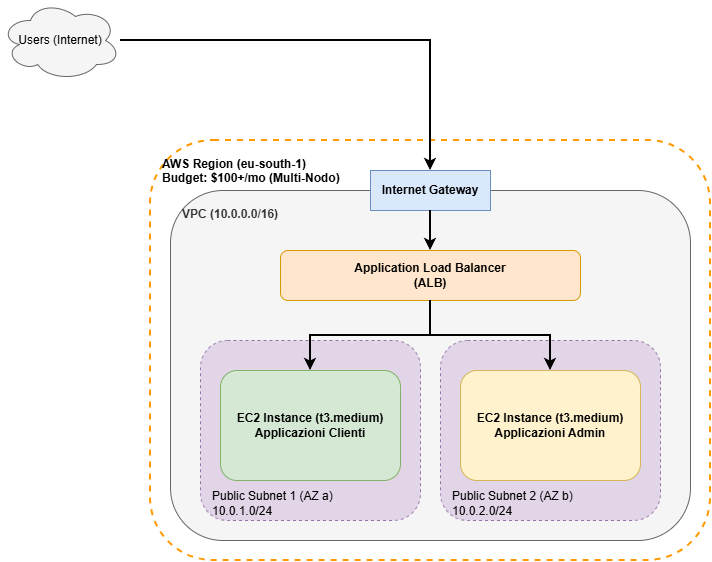
\includegraphics[width=0.9\textwidth]{img/AWSArchitecture.png}
    \caption{Schema Architetturale AWS Multi-Nodo (VPC, Subnet, EC2, ALB)}
    \label{fig:aws_arch}
\end{figure}

\textbf{Load Balancing e Path-Based Routing:}\\
Al fine di separare le competenze mantenendo un singolo punto d'accesso, l'Application Load Balancer (ALB) è stato configurato per effettuare un \textit{Path-Based Routing}. Il traffico in entrata viene analizzato dall'ALB: le richieste dirette ai path \texttt{/admin*} e \texttt{/inventory*} vengono inoltrate automaticamente al \textit{Target Group} del nodo Admin (situato nella Subnet 2), mentre tutte le restanti richieste (di default) sono servite dal \textit{Target Group} del nodo Clienti (nella Subnet 1).

\textbf{Nota sulla configurazione delle credenziali IAM per Terraform:}\\
Per consentire a Terraform di effettuare il provisioning delle risorse su AWS, è necessario configurare correttamente un utente programmatico tramite IAM (Identity and Access Management). Seguendo le best practice illustrate nei tutorial di riferimento (come l'aggiunta dell'utente a un Gruppo IAM specifico), si consiglia di applicare al gruppo la policy predefinita \texttt{AdministratorAccess}. 
Considerando che lo script Terraform necessita di orchestrare contemporaneamente VPC, Security Group, Istanze EC2, Application Load Balancer e impostazioni di Billing (per l'allarme budget), l'accesso amministratore garantisce un'esecuzione senza blocchi o errori di permessi per scopi didattici e di test. In scenari di produzione reali, tuttavia, andrebbe rigorosamente applicato il principio del privilegio minimo (Least Privilege), assemblando policy granulari (ad es. \texttt{AmazonEC2FullAccess}, \texttt{AmazonVPCFullAccess}, ecc.).

\textbf{Selezione dello Use Case per l'Access Key:}\\
Durante la procedura guidata di generazione della coppia di chiavi di accesso (\textit{Access Key} e \textit{Secret Access Key}) nella AWS Console, viene richiesto di specificare l'ambito di utilizzo (\textit{Use case}):
\begin{itemize}
    \item L'opzione da selezionare è \textbf{Command Line Interface (CLI)}. Terraform, infatti, opera interfacciandosi con le API di AWS esattamente come un tool a riga di comando locale (o caricando le credenziali tramite l'AWS CLI configurata con \texttt{aws configure}, oppure leggendo i file \texttt{.aws/credentials} o variabili d'ambiente).
    \item Spuntando la casella di conferma relativa alle raccomandazioni di sicurezza AWS ("I understand the above recommendation and want to proceed..."), è possibile procedere con la generazione e il download del file \texttt{.csv} contenente le chiavi.
\end{itemize}

I passi per eseguire lo script sono i seguenti:
\begin{enumerate}
    \item \textbf{Configurazione Credenziali:} Eseguire \texttt{aws configure} per configurare la CLI con le \textit{Access Keys} ottenute.
    \begin{figure}[H]
        \centering
        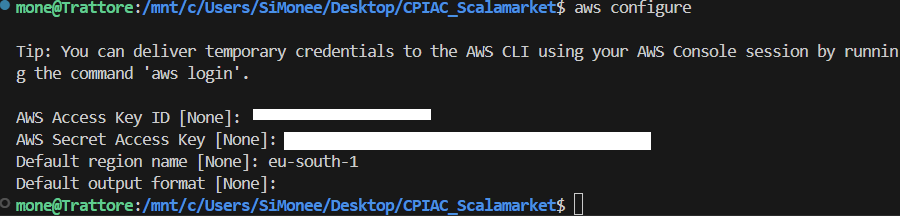
\includegraphics[width=0.7\textwidth]{img/awsConfigure.png}
        \caption{Configurazione tramite AWS CLI}
        \label{fig:aws_configure}
    \end{figure}
    \item \textbf{Inizializzazione:} Eseguire \texttt{terraform init}.
    \begin{figure}[H]
        \centering
        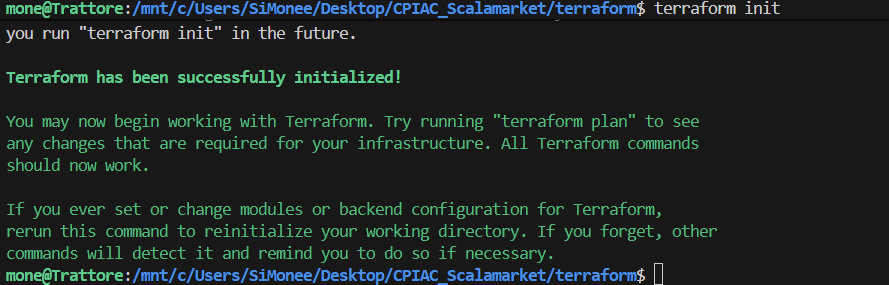
\includegraphics[width=0.7\textwidth]{img/terraformInit.png}
        \caption{Inizializzazione di Terraform}
        \label{fig:terraform_init}
    \end{figure}
    \item \textbf{Verifica e Applicazione:} Eseguire \texttt{terraform plan} e infine \texttt{terraform apply}.
    \begin{figure}[H]
        \centering
        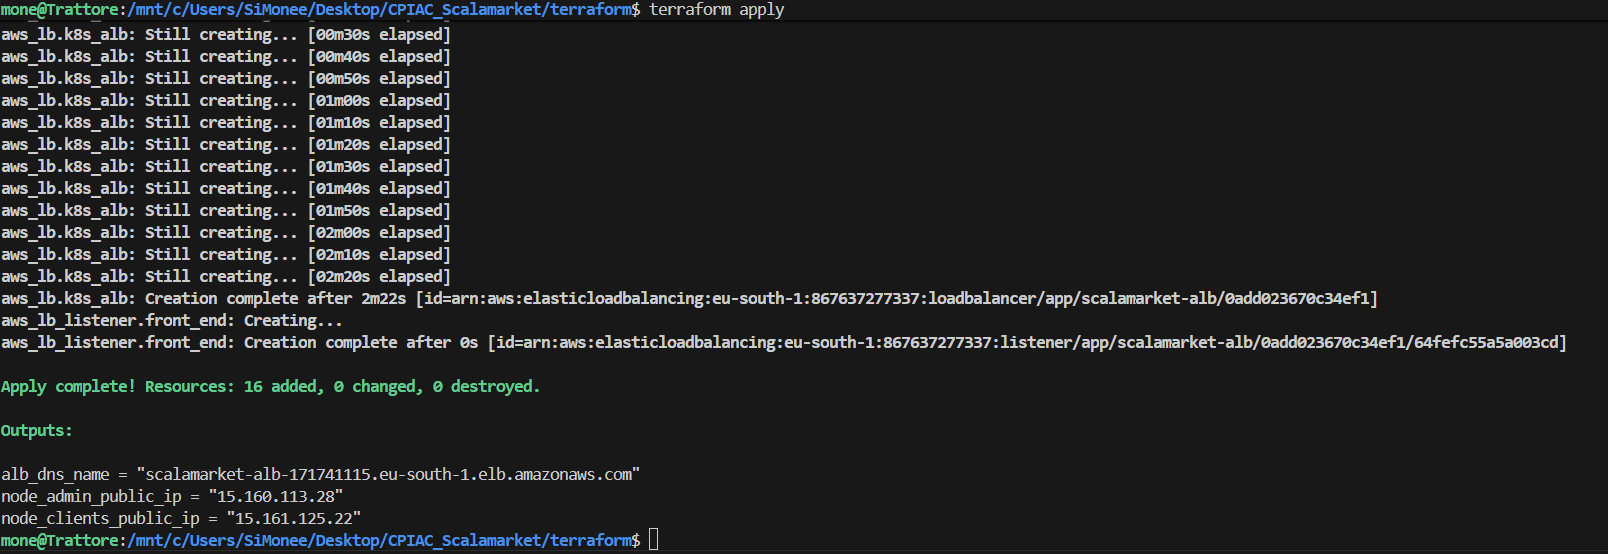
\includegraphics[width=0.7\textwidth]{img/TerraformApply.png}
        \caption{Output del comando Terraform Apply}
        \label{fig:terraform_apply}
    \end{figure}
\end{enumerate}

\textbf{Accesso Remoto e Deploy Applicativo:}\\
Al termine dell'esecuzione di Terraform, verranno stampati a video il DNS name dell'ALB e gli IP Pubblici delle due istanze EC2. 
L'infrastruttura a questo punto è in esecuzione, ma le applicazioni devono ancora essere deployate. I passaggi sono:
\begin{itemize}
    \item \textbf{Accesso SSH:} Collegarsi in SSH alle macchine tramite la chiave definita (es. \texttt{scalamarket-key}).
    \item \textbf{Clone Selettivo (Sparse-Checkout):} Per evitare di scaricare file inutili ai fini del deploy (come questa documentazione o i file Terraform), utilizzare i seguenti comandi su entrambi i nodi:
    \begin{verbatim}
    git clone --no-checkout <TUO_URL_GIT>
    cd CPIAC_Scalamarket
    git sparse-checkout init --cone
    git sparse-checkout set frontend init-scripts microservices k8s
    git checkout main
    \end{verbatim}
    \item \textbf{Deploy K8s - Nodo Clienti:} (Assicurarsi di essere nella cartella \texttt{CPIAC\_Scalamarket})
    \begin{verbatim}
    sudo docker build -t cpiac_frontend:v5 -f frontend/Dockerfile frontend/
    sudo docker build -t cpiac_auth:v5    -f microservices/auth_service/Dockerfile .
    sudo docker build -t cpiac_order:v5   -f microservices/order_service/Dockerfile .

    sudo kubectl apply -f k8s/postgres-pv-pvc.yaml
    sudo kubectl apply -f k8s/postgres-configmap.yaml
    sudo kubectl apply -f k8s/postgres-deployment.yaml
    sudo kubectl apply -f k8s/postgres-service.yaml

    sudo kubectl apply -f k8s/frontend-deployment.yaml
    sudo kubectl apply -f k8s/frontend-service.yaml
    sudo kubectl apply -f k8s/auth-deployment.yaml
    sudo kubectl apply -f k8s/auth-service.yaml
    sudo kubectl apply -f k8s/order-deployment.yaml
    sudo kubectl apply -f k8s/order-service.yaml
    sudo kubectl apply -f k8s/ingress.yaml
    \end{verbatim}
    
    \item \textbf{Deploy K8s - Nodo Admin:}
    \begin{verbatim}
    sudo docker build -t cpiac_inventory:v5 -f microservices/inventory_service/Dockerfile .

    sudo kubectl apply -f k8s/postgres-pv-pvc.yaml
    sudo kubectl apply -f k8s/postgres-configmap.yaml
    sudo kubectl apply -f k8s/postgres-deployment.yaml
    sudo kubectl apply -f k8s/postgres-service.yaml

    sudo kubectl apply -f k8s/inventory-deployment.yaml
    sudo kubectl apply -f k8s/inventory-service.yaml
    sudo kubectl apply -f k8s/ingress.yaml
    \end{verbatim}
    \item \textbf{Navigazione:} Accedere dal browser non tramite gli IP delle macchine, ma tramite l'URL fornito dall'Application Load Balancer (DNS Name). L'ALB smisterà automaticamente il traffico basandosi sul \textit{path} dell'URL.
\end{itemize}
\end{mysection}

\begin{mysection}{Deployment tramite AWS Management Console (GUI)}
In alternativa, è possibile creare manualmente la stessa infrastruttura descritta al paragrafo precedente direttamente tramite il portale web di AWS. Questo approccio è utile a scopo esplorativo e didattico.

Di seguito i passaggi principali:
\begin{enumerate}
    \item \textbf{Creazione VPC:} Dalla sezione VPC, utilizzare il wizard "VPC and more" per creare la rete, specificando il CIDR block e includendo un Internet Gateway.
    \item \textbf{Configurazione Subnet e Route Table:} Separare logicamente le reti pubbliche e private.
    \item \textbf{Lancio Istanze EC2:} Dalla dashboard EC2, cliccare su "Launch Instance". Selezionare un'AMI Ubuntu, scegliere una classe di istanza (es. \texttt{t3.medium}), associare una coppia di chiavi SSH e collocare l'istanza nella subnet corretta associandole un Security Group che apra la porta 22 (SSH) e la 80 (HTTP).
    \item \textbf{Creazione Load Balancer:} Dalla sezione "Load Balancing", creare un ALB, associarlo alle subnet pubbliche e creare un \textit{Target Group} che punti alle istanze EC2 su cui gira Kubernetes.
    \item \textbf{Impostazione AWS Budget:} Dalla sezione "Billing", accedere a "Budgets" e creare un budget di costo mensile pari a 100\$, specificando l'indirizzo email per gli alert al superamento dell'80\%.
\end{enumerate}



\end{mysection}

\end{mychapter}
